%\documentclass[lang=en,aspectratio=43]{mupresentation}
\documentclass[lang=eu,biz=pls,aspectratio=169,handout]{mupresentation}

\title{Devcontainer-ak\\Informatika Graduan}
\subtitle{INFOR Ekimenak}
\institute{Mondragon Unibertsitatea}
\date{}
\version{v2.0.0}

\usepackage{tikz}

\begin{document}

\mucover

\begin{frame}
  \frametitle{Zer da Devcontainer bat?}
  \begin{itemize}
    \item Software \textbf{garapena} egiteko behar den ingurunea barnean dakarren \textit{Docker} \textbf{Container} bat da.
    \item Visual Studio Code-ren zerbitzari zatia Container \textbf{barruan} exekutatzen da.
    \item Garatzailea bere sistema eragilean duen Visual Studio Code-rekin konektatu daiteke bezero gisa. Horrela, \textbf{garapena Container-ean} egon balitz bezala egiten da.
    \item Hasieran Microsoftek bultzatu zuen baina orain espezifikazio \textbf{ireki} bat da:
      \url{https://containers.dev/}
  \end{itemize}
\end{frame}

\begin{frame}
  \frametitle{Demo time!}
\end{frame}

\begin{frame}
  \frametitle{The Good: Garrantzia graduan}
  \begin{itemize}
    \item Ikasleek eta irakasleek \textbf{hainbat} garapen-ingurune erabili behar dituzte graduan zehar. Ikasgai ezberdinak, transferentzia proiektuak, ikerketa, ...
    \item Devcontainer-ek ingurune hauek elkarren artean \textbf{bereizten} laguntzen dute.
    \begin{itemize}
      \item Bertsio ezberdinen arteko \textbf{talkak ekiditen} laguntzen dute.
    \end{itemize}
    \item Devcontainer-ek \textbf{ez dute} gure sistema eragilea (\textit{hosta}) \textbf{aldatzen}.
    \item \textbf{Erreplikagarriak} dira. Ikasleek eta irakasleek ingurune berdina izan dezaten laguntzen dute.
  \end{itemize}
\end{frame}

\begin{frame}
  \frametitle{Zer egin dugu?}
  \begin{itemize}
    \item Devcontainer-ei buruzko \textbf{git biltegi} bat sortu dugu:
      \url{https://gitlab.com/mu-bd-ce/devcontainers}.

      Bertan aurkituko ditugu:
      \begin{itemize}
        \item Programazio lengoaia ezberdinendako \textbf{aurrez-sorturiko Devcontainer-ak}. Adibidez:
          \url{registry.gitlab.com/mu-bd-ce/devcontainers/python:latest}
        \item Hauei buruzko \textbf{dokumentazioa}:
          \url{https://mu-bd-ce.gitlab.io/devcontainers}
        \item Hauek nola erabili azaltzen duten \textbf{adibideak}.
      \end{itemize}
    \item Bigarren mailako web eta estatistika ikasgaietan \textbf{lehenengo saiakera} egin dugu.
  \end{itemize}
\end{frame}

\begin{frame}
  \frametitle{The bad}
  \begin{itemize}
    \item Arazoa (The bad): I/O errendimendua Windows-en. Lan eremua windows-en badago sarrera irteera operazioak asko moteldu daitezke.
  \end{itemize}
  \vspace{1em}
  \centering
  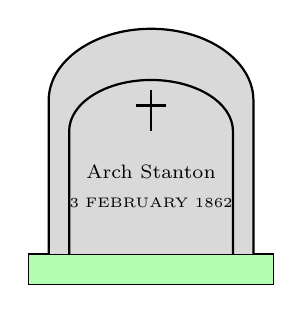
\begin{tikzpicture}[scale=1.3]
    % Ground
    \draw[fill=green!30] (-0.2,0.2) rectangle (2.2,0.5);
    % Grave
    \draw[thick, fill=gray!30] (0,0.5) -- (0,2) arc (180:0:1 and 0.7) -- (2,0.5);
    \draw[thick] (0.2,0.5) -- (0.2,1.7) arc (180:0:0.8 and 0.5) -- (1.8,0.5);
    % R.I.P. text
    \node at (1,1.3) {\scriptsize Arch Stanton};
    \node at (1,1) {\tiny 3 FEBRUARY 1862};
    % Cross
    \draw[thick] (1,1.7) -- (1,2.1);
    \draw[thick] (0.85,1.95) -- (1.15,1.95);
  \end{tikzpicture}
\end{frame}

\begin{frame}
  \frametitle{Devcontainer-ak Windows-en}
  \centering
  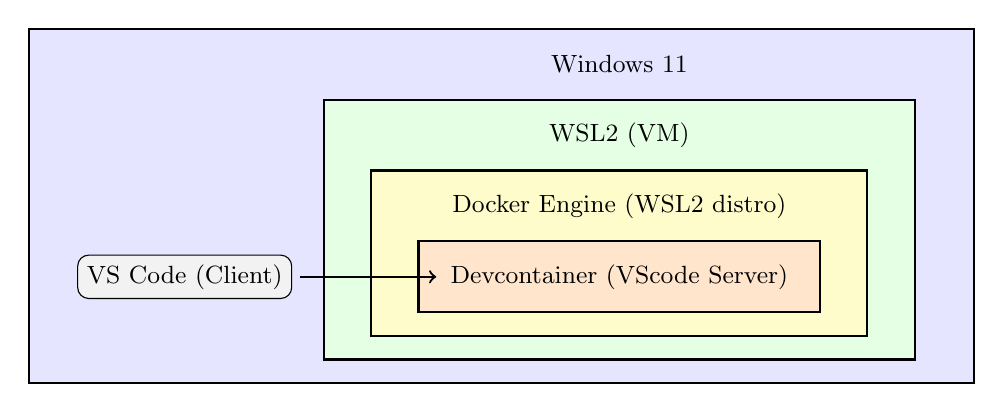
\begin{tikzpicture}[scale=1.5, every node/.style={font=\small}]
    % Windows box
    \draw[thick, fill=blue!10] (-2,0) rectangle (6,3);
    \node at (3,2.7) {Windows 11};
    % WSL box inside Windows
    \draw[thick, fill=green!10] (0.5,0.2) rectangle (5.5,2.4);
    \node at (3,2.1) {WSL2 (VM)};
    % Docker inside WSL
    \draw[thick, fill=yellow!20] (0.9,0.4) rectangle (5.1,1.8);
    \node at (3,1.5) {Docker Engine (WSL2 distro)};
    % Devcontainer inside Docker
    \draw[thick, fill=orange!20] (1.3,0.6) rectangle (4.7,1.2);
    \node at (3,0.9) {Devcontainer (VScode Server)};
    % VS Code outside, arrow to Devcontainer
    \node[draw, fill=gray!10, rounded corners] at (-0.68,0.9) {VS Code (Client)};
    \draw[->, thick] (0.3,0.9) -- (1.45,0.9);
  \end{tikzpicture}
\end{frame}

\begin{frame}
  \frametitle{The ugly}
  \begin{itemize}
    \item Konponbideak:
      \begin{itemize}
        \item Devcontainer-ak \textbf{Linux} sistemetan erabiltzea.
        \item Windows-en, WSL2 eta Docker Desktop erabiltzea.
      \end{itemize}
  \end{itemize}
  \vspace{1em}
  \centering
  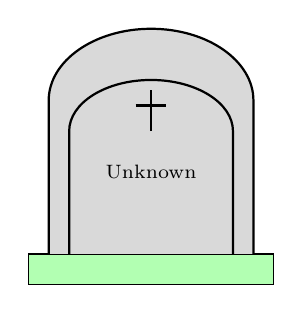
\begin{tikzpicture}[scale=1.3]
    % Ground
    \draw[fill=green!30] (-0.2,0.2) rectangle (2.2,0.5);
    % Grave
    \draw[thick, fill=gray!30] (0,0.5) -- (0,2) arc (180:0:1 and 0.7) -- (2,0.5);
    \draw[thick] (0.2,0.5) -- (0.2,1.7) arc (180:0:0.8 and 0.5) -- (1.8,0.5);
    % R.I.P. text
    \node at (1,1.3) {\scriptsize Unknown};
    % Cross
    \draw[thick] (1,1.7) -- (1,2.1);
    \draw[thick] (0.85,1.95) -- (1.15,1.95);
  \end{tikzpicture}
\end{frame}

\begin{frame}
  \frametitle{Gure Proposamena}
  \begin{itemize}
    \item Hurrengo kurtsoan ekimen honetara \textbf{ikasgai gehiago batzea}.
    \item Git biltegia graduan erabiltzen ditugun \textbf{teknologiak estandarizatzeko} erabiltzea (adibidez, graduko Java bertsioa) \footnote{Biltegi hau lehenengo hurbilketa da; Devcontainer hauen alderdi guztiak eztabaidatzeko \textbf{irekita} daude.}.
  \end{itemize}
\end{frame}

\begin{frame}
  \frametitle{Three more things...}
  \begin{itemize}
    \item Github Codespaces: .
    \item MU LaTeX template: \url{https://gitlab.com/mu-bd-ce/mu-latex-template}.
    \item Github Copilot: GPT-4.1 eta GPT-4o doahinik. Github Education-ekin Premium modeloak (Claude Sonnet 4, ...).
  \end{itemize}
\end{frame}

\muback{Eskerrik asko}{Ibai Roman\\
  Software \& System Engineering\\
  Electronics and Computer Science department\\
  Mondragon Unibertsitatea - Faculty of Engineering\\
\href{www.mondragon.edu}{www.mondragon.edu}}

\end{document}